\documentclass{beamer}
\mode<presentation>
\usepackage{amsmath,amssymb,mathtools}
\usepackage{textcomp}
\usepackage{gensymb}
\usepackage{adjustbox}
\usepackage{subcaption}
\usepackage{enumitem}
\usepackage{multicol}
\usepackage{listings}
\usepackage{url}
\usepackage{graphicx} % <-- needed for images
\def\UrlBreaks{\do\/\do-}

\usetheme{Boadilla}
\usecolortheme{lily}
\setbeamertemplate{footline}{
  \leavevmode%
  \hbox{%
  \begin{beamercolorbox}[wd=\paperwidth,ht=2ex,dp=1ex,right]{author in head/foot}%
    \insertframenumber{} / \inserttotalframenumber\hspace*{2ex}
  \end{beamercolorbox}}%
  \vskip0pt%
}
\setbeamertemplate{navigation symbols}{}

\lstset{
  frame=single,
  breaklines=true,
  columns=fullflexible,
  basicstyle=\ttfamily\tiny   % tiny font so code fits
}

\numberwithin{equation}{section}

% ---- your macros ----
\providecommand{\nCr}[2]{\,^{#1}C_{#2}}
\providecommand{\nPr}[2]{\,^{#1}P_{#2}}
\providecommand{\mbf}{\mathbf}
\providecommand{\pr}[1]{\ensuremath{\Pr\left(#1\right)}}
\providecommand{\qfunc}[1]{\ensuremath{Q\left(#1\right)}}
\providecommand{\sbrak}[1]{\ensuremath{{}\left[#1\right]}}
\providecommand{\lsbrak}[1]{\ensuremath{{}\left[#1\right.}}
\providecommand{\rsbrak}[1]{\ensuremath{\left.#1\right]}}
\providecommand{\brak}[1]{\ensuremath{\left(#1\right)}}
\providecommand{\lbrak}[1]{\ensuremath{\left(#1\right.}}
\providecommand{\rbrak}[1]{\ensuremath{\left.#1\right)}}
\providecommand{\cbrak}[1]{\ensuremath{\left\{#1\right\}}}
\providecommand{\lcbrak}[1]{\ensuremath{\left\{#1\right.}}
\providecommand{\rcbrak}[1]{\ensuremath{\left.#1\right\}}}
\theoremstyle{remark}
\newtheorem{rem}{Remark}
\newcommand{\sgn}{\mathop{\mathrm{sgn}}}
\providecommand{\abs}[1]{\left\vert#1\right\vert}
\providecommand{\res}[1]{\Res\displaylimits_{#1}}
\providecommand{\norm}[1]{\lVert#1\rVert}
\providecommand{\mtx}[1]{\mathbf{#1}}
\providecommand{\mean}[1]{E\left[ #1 \right]}
\providecommand{\fourier}{\overset{\mathcal{F}}{ \rightleftharpoons}}
\providecommand{\system}{\overset{\mathcal{H}}{ \longleftrightarrow}}
\providecommand{\dec}[2]{\ensuremath{\overset{#1}{\underset{#2}{\gtrless}}}}
\newcommand{\myvec}[1]{\ensuremath{\begin{pmatrix}#1\end{pmatrix}}}
\let\vec\mathbf

\title{MatGeo Presentation - Problem 8.2.32}
\author{EE25BTECH11064 - Yojit Manral}
\date{}

\begin{document}

\frame{\titlepage}
\begin{frame}{Question}
Find the conic equation that satisfies the given conditions: ends of the major axis $(0,\pm5)$, ends of the minor axis $(\pm1,0)$.
\end{frame}

\begin{frame}{Solution}
$\rightarrow$ The equation for any conic having directrix $\vec{n}^T\vec{x}=c$ and eccentricity $e$ is given by
\begin{align}
    \vec{x}^T\vec{V}\vec{x} + 2\vec{u}^T\vec{x} + f = 0 \\
    \vec{V} = \norm{\vec{n}}^2\vec{I}-e^2\vec{n}\vec{n}^T
\end{align}
$\rightarrow$ As the major axis is along the $Y-axis$
\begin{align} \vec{n} = \vec{e_2} \implies \vec{V} = \myvec{1&0\\0&1-e^2} \end{align}
$\rightarrow$ Also, as the center of the ellipse is at origin
\begin{align} \vec{C} = 0 \implies \vec{u} = 0 \end{align}
$\rightarrow$ Let $\vec{P}$ and $\vec{Q}$ be points on the ellipse
\begin{align} \vec{P} = \myvec{1\\0} && \vec{Q} = \myvec{0\\5} \end{align}
\end{frame}

\begin{frame}{Solution}
$\rightarrow$ Then, $\vec{P}$ and $\vec{Q}$ satisfy (1)
\begin{align}
    \vec{P}^T\vec{V}\vec{P} + 2\vec{u}^T\vec{P} + f = 0 && \vec{Q}^T\vec{V}\vec{Q} + 2\vec{u}^T\vec{Q} + f = 0 \\
    \myvec{1&0}\myvec{1&0\\0&1-e^2}\myvec{1\\0} = -f && \myvec{0&5}\myvec{1&0\\0&1-e^2}\myvec{0\\5} = -f \\
    1 = -f && 25(1-e^2) = -f\\
    f = -1 && \implies e^2 = 1+\frac{f}{25} = \frac{24}{25}
\end{align}
$\rightarrow$ Thus, we get the equation of the conic as
\begin{align}
    \vec{V}=\myvec{1&0\\0&1-e^2}=\myvec{1&0\\0&1/25} \text{, } \vec{u}&=0 \text{, and } f=-1\\
    \implies \vec{x}^T\myvec{1&0\\0&1/25}\vec{x} - 1 &= 0
\end{align}
\end{frame}

\begin{frame}{Solution}
\begin{figure}[h!]
   \centering
   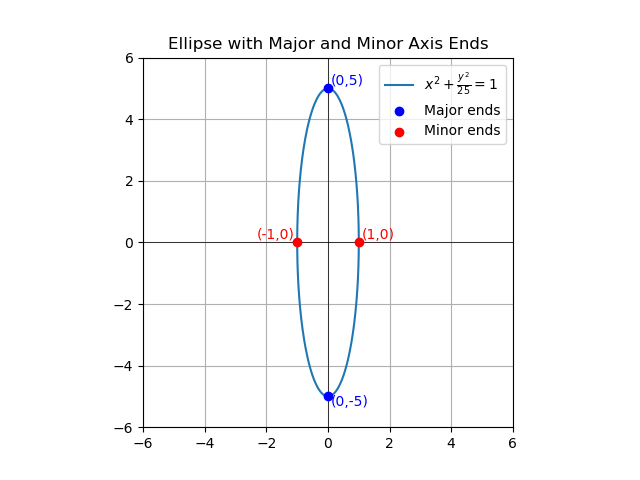
\includegraphics[width=0.8\linewidth]{figs/01.png}
   \caption{Plot of required conic}
   \label{Plot_1}
\end{figure}
\end{frame}
 % --------- CODE APPENDIX ---------
\section*{Appendix: Code}

% C program
\begin{frame}[fragile]{File: points.c}
\begin{lstlisting}[language=C]
#include <stdio.h>

int main() {
  FILE *fp;

  // -------------------
  // Question 8.2.32
  // -------------------


  fp = fopen("points.dat", "w");
  fprintf(fp, "%d,%d,%d\n", 0, 5, 0); // A
  fprintf(fp, "%d,%d,%d\n", 1, 0, 0); // B
  fprintf(fp, "%d,%d,%d\n", 0, -5, 0); // C
  fprintf(fp, "%d,%d,%d\n", -1, 0, 0); // D
  fclose(fp);
  return 0;
}
\end{lstlisting}
\end{frame}

% Python calling C
\begin{frame}[fragile]{File: call\_c.py}
\begin{lstlisting}[language=Python]
import subprocess

# Compile the C program
subprocess.run(["gcc", "points.c", "-o", "points"])

# Run the compiled C program
result = subprocess.run(["./points"], capture_output=True, text=True)

# Print the output from the C program
print(result.stdout)
\end{lstlisting}
\end{frame}

% Python plotting
\begin{frame}[fragile]{File: plot.py}
\begin{lstlisting}[language=Python]
import numpy as np
import matplotlib.pyplot as plt

# Parameters of the ellipse
a = 5  # semi-major axis
b = 1  # semi-minor axis

# Parametric equations of ellipse
theta = np.linspace(0, 2*np.pi, 400)
y = a * np.sin(theta)
x = b * np.cos(theta)

# Plot ellipse
plt.plot(x, y, label=r"$x^2+\frac{y^2}{25}=1$")

# Mark ends of the axes
plt.scatter([0, 0], [5, -5], color="blue", zorder=5, label="Major ends")
plt.scatter([1, -1], [0, 0], color="red", zorder=5, label="Minor ends")
plt.text(1.1, 0.1, "(1,0)", color="red")
plt.text(-2.3, 0.1, "(-1,0)", color="red")
plt.text(0.1, 5.1, "(0,5)", color="blue")
plt.text(0.1, -5.3, "(0,-5)", color="blue")

# Axes setup
plt.axhline(0, color="black", linewidth=0.5)
plt.axvline(0, color="black", linewidth=0.5)
plt.gca().set_aspect('equal')
plt.legend(loc='upper right')
plt.title("Ellipse with Major-Axis and Minor-Axis Ends")
plt.xlim(-6, 6)
plt.ylim(-6, 6)
plt.grid(True)
plt.show()
\end{lstlisting}
\end{frame}

\end{document}
